\section{Flüssigkristalle}
Flüssigkristalle haben zwischen den Aggregatzuständen ``fest'' und ``flüssig'' einen weiteren Aggregatzustand: 
Der ``flüssigkristalline'' Aggregatzustand macht sich erkennbar durch die trübe Farbe. Hauptursache: ZMK   

Es werden 3 verschiedene flüssigkristalline Phasen unterschieden:
\begin{itemize}
    \item smektische Phase (kein Vorbeigleiten, Schichten)
    \item nematische Phase (Vorbeigleiten möglich, nicht geordnet)
    \item cholesterische Phase (Schichten mit nem. Phase, jede Schicht vedreht)
\end{itemize}
Damit Moleküle eine solche Phase zeigen können, müssen folgende Kriterien erfüllt sein:
\begin{itemize}
    \item lange, stäbchenartige Moleküle (4x - 6x Molekülbreite)
    \item starre Atomgruppen wie z.B. Benzol-Ringe, Doppel-, Dreifachbindungen
    \item funktionelle Gruppe mit sehr starkem Dipolmoment (-CN-, -COOH)
\end{itemize}
% \vspace{-0.2cm}
% \begin{center}
%     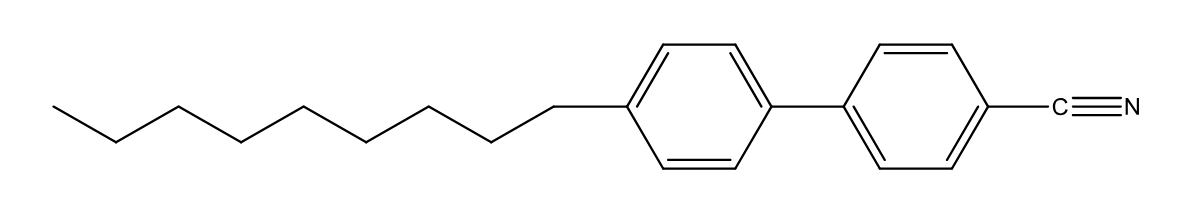
\includegraphics[height=1cm]{pictures/CN-Fluessigkrist.png}
% \end{center}
% \vspace{-0.5cm}

\subsection{TN-Zelle (Twisted Nematic)}
\begin{minipage}{0.48\linewidth}
    \begin{center}
        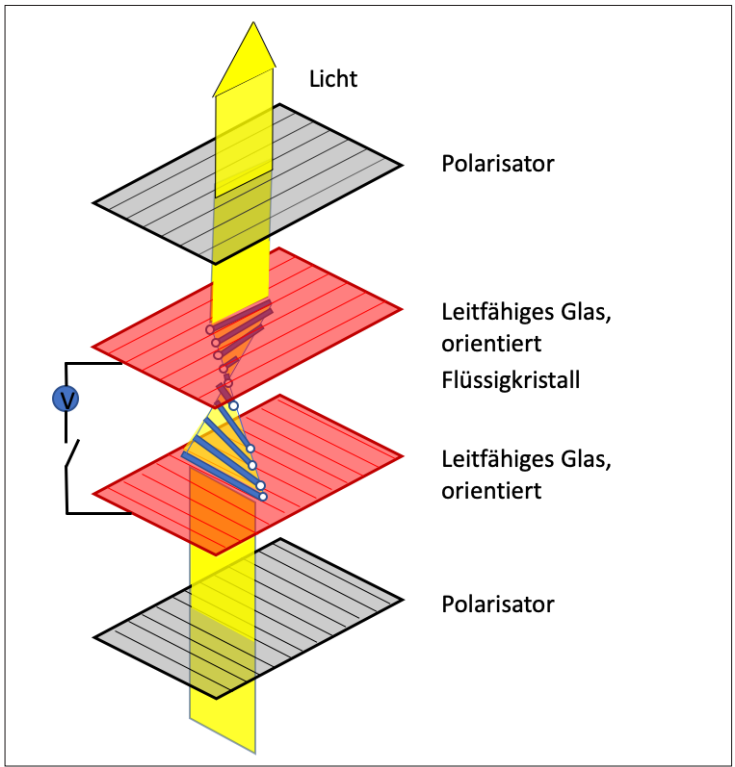
\includegraphics[width=0.8\linewidth]{pictures/TN-Zelle1.png}
    
        ohne angelegte Spannung   
    \end{center}
\end{minipage}
\hfill
\begin{minipage}{0.48\linewidth}
    \begin{center}
        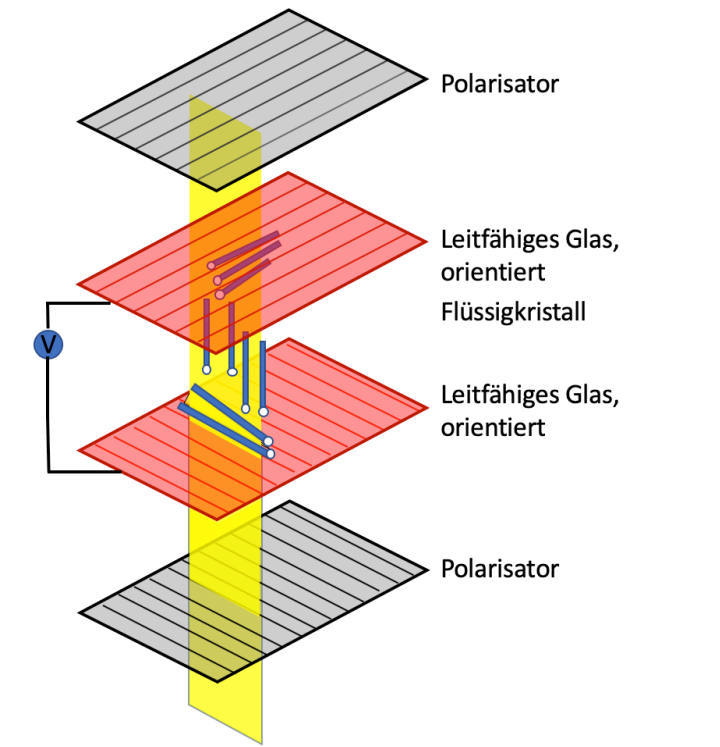
\includegraphics[width=0.8\linewidth]{pictures/TN-Zelle2.png} 
    
        mit angelegter Spannung 
    \end{center}
\end{minipage}

